\section{Bond Graphs}
\begin{figure}[H]
    \centering
    \begin{minipage}{.5\textwidth}
        \centering
        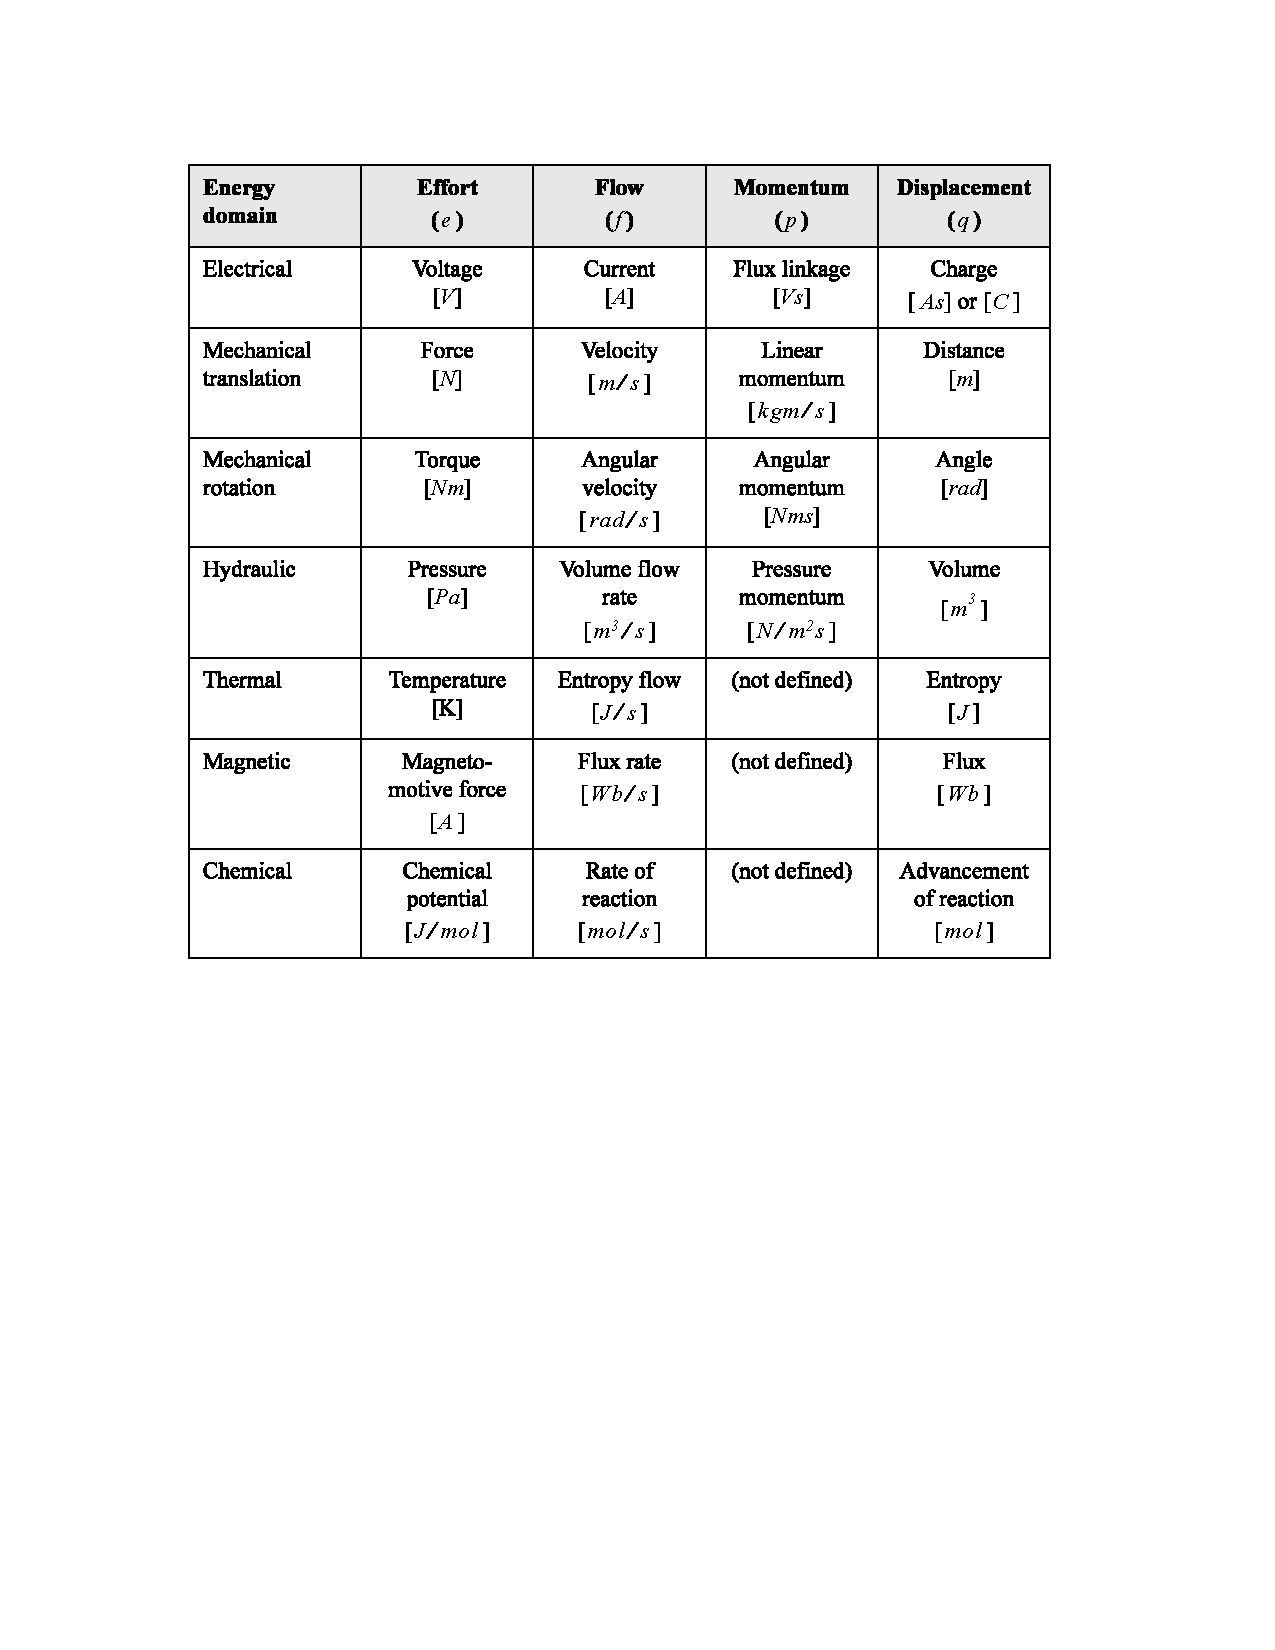
\includegraphics[width=.9\linewidth]{figures/Tabell_EnergyDomain.pdf}
        \label{fig:bond_graph1}
        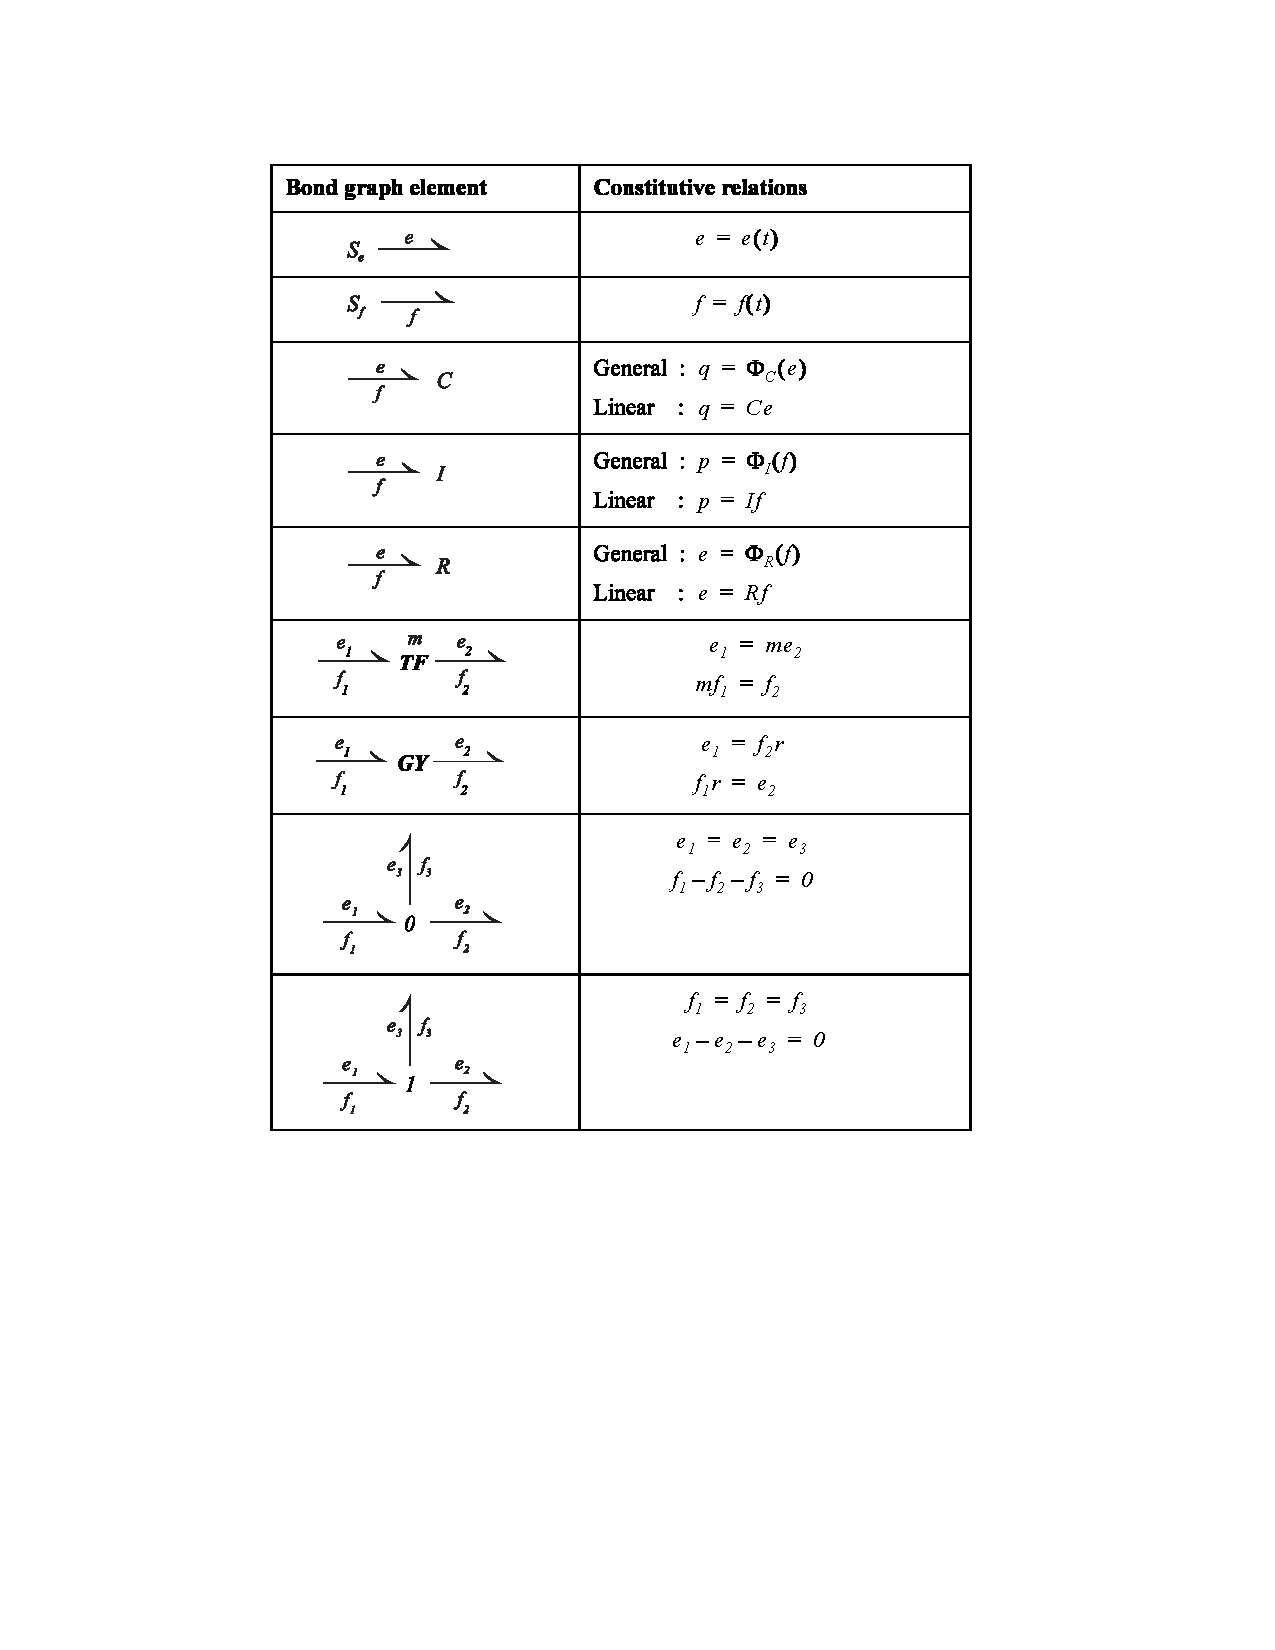
\includegraphics[width=.9\linewidth]{figures/Tabell_GraphElements.pdf}
        \label{fig:bond_graph2}
    \end{minipage}%
    \begin{minipage}{.5\textwidth}
        \centering
        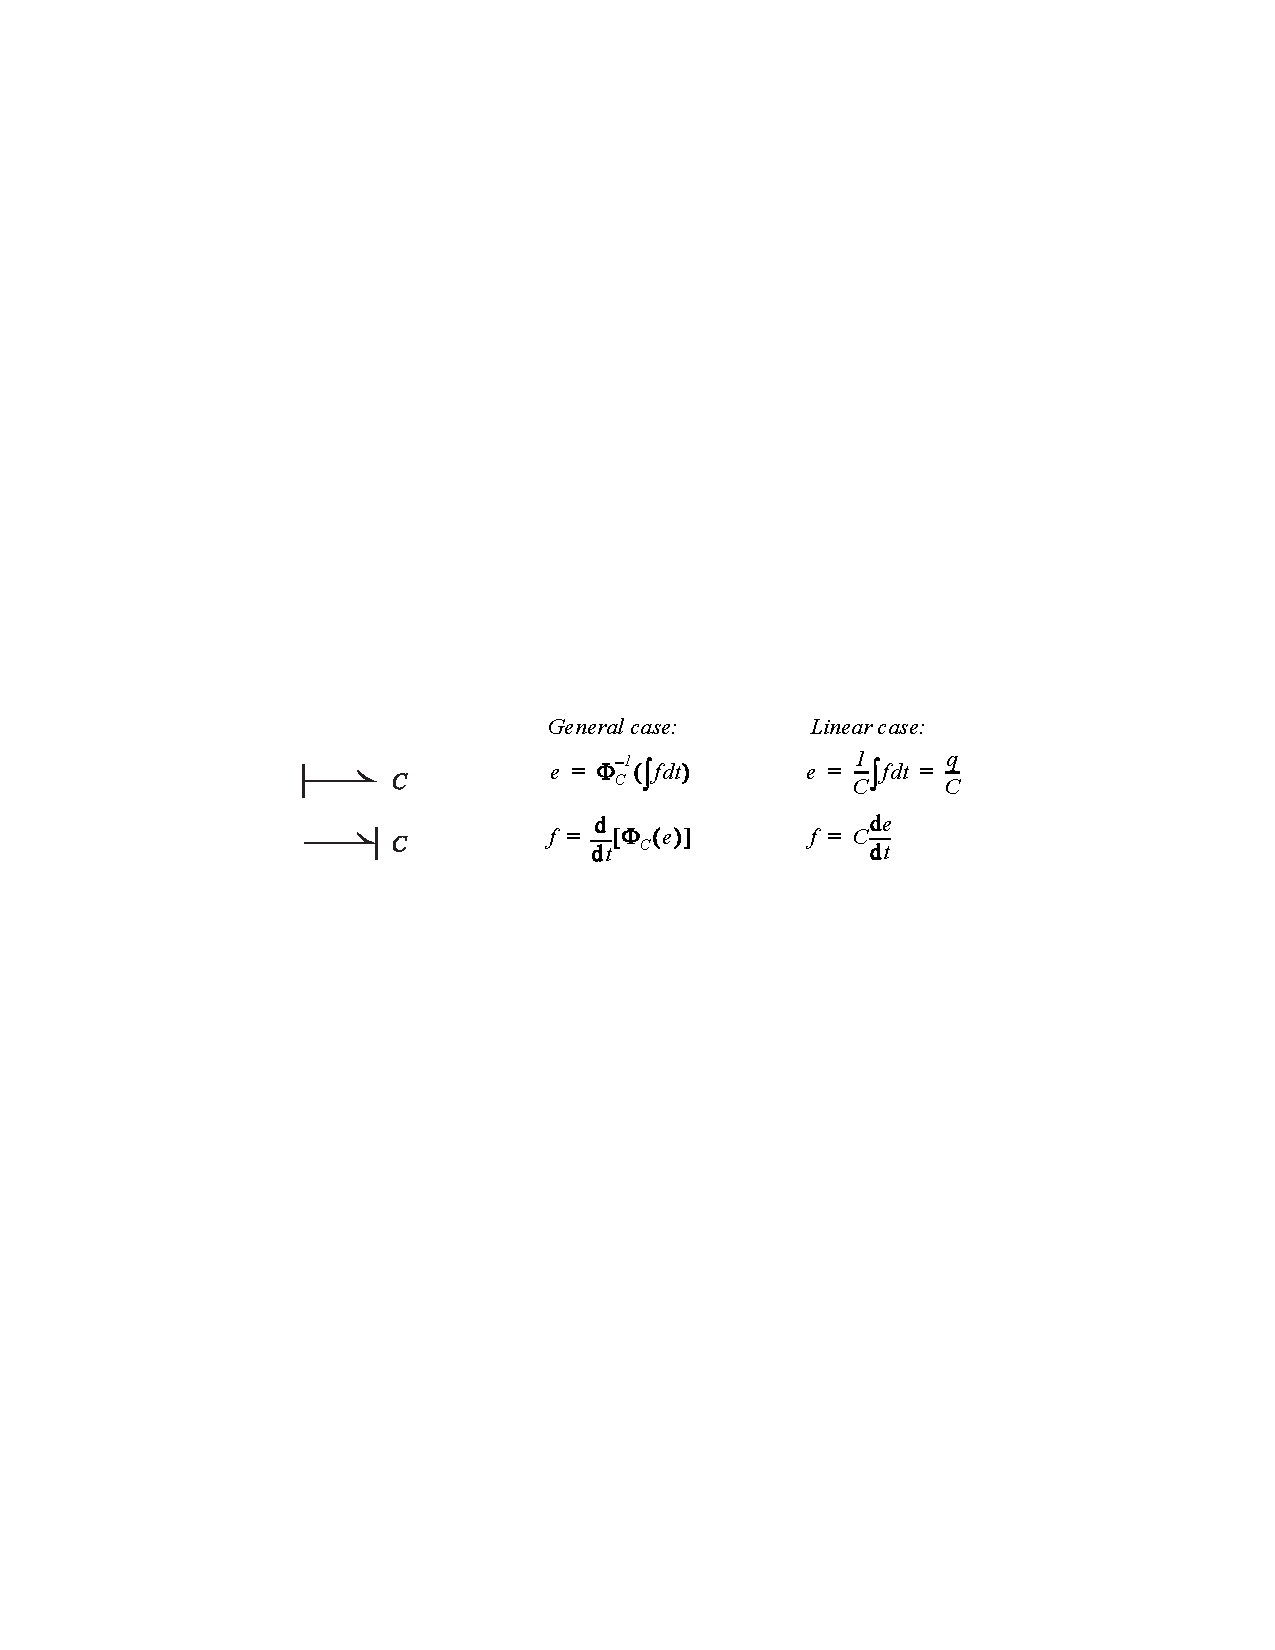
\includegraphics[width=.9\linewidth]{figures/fig45.pdf}
        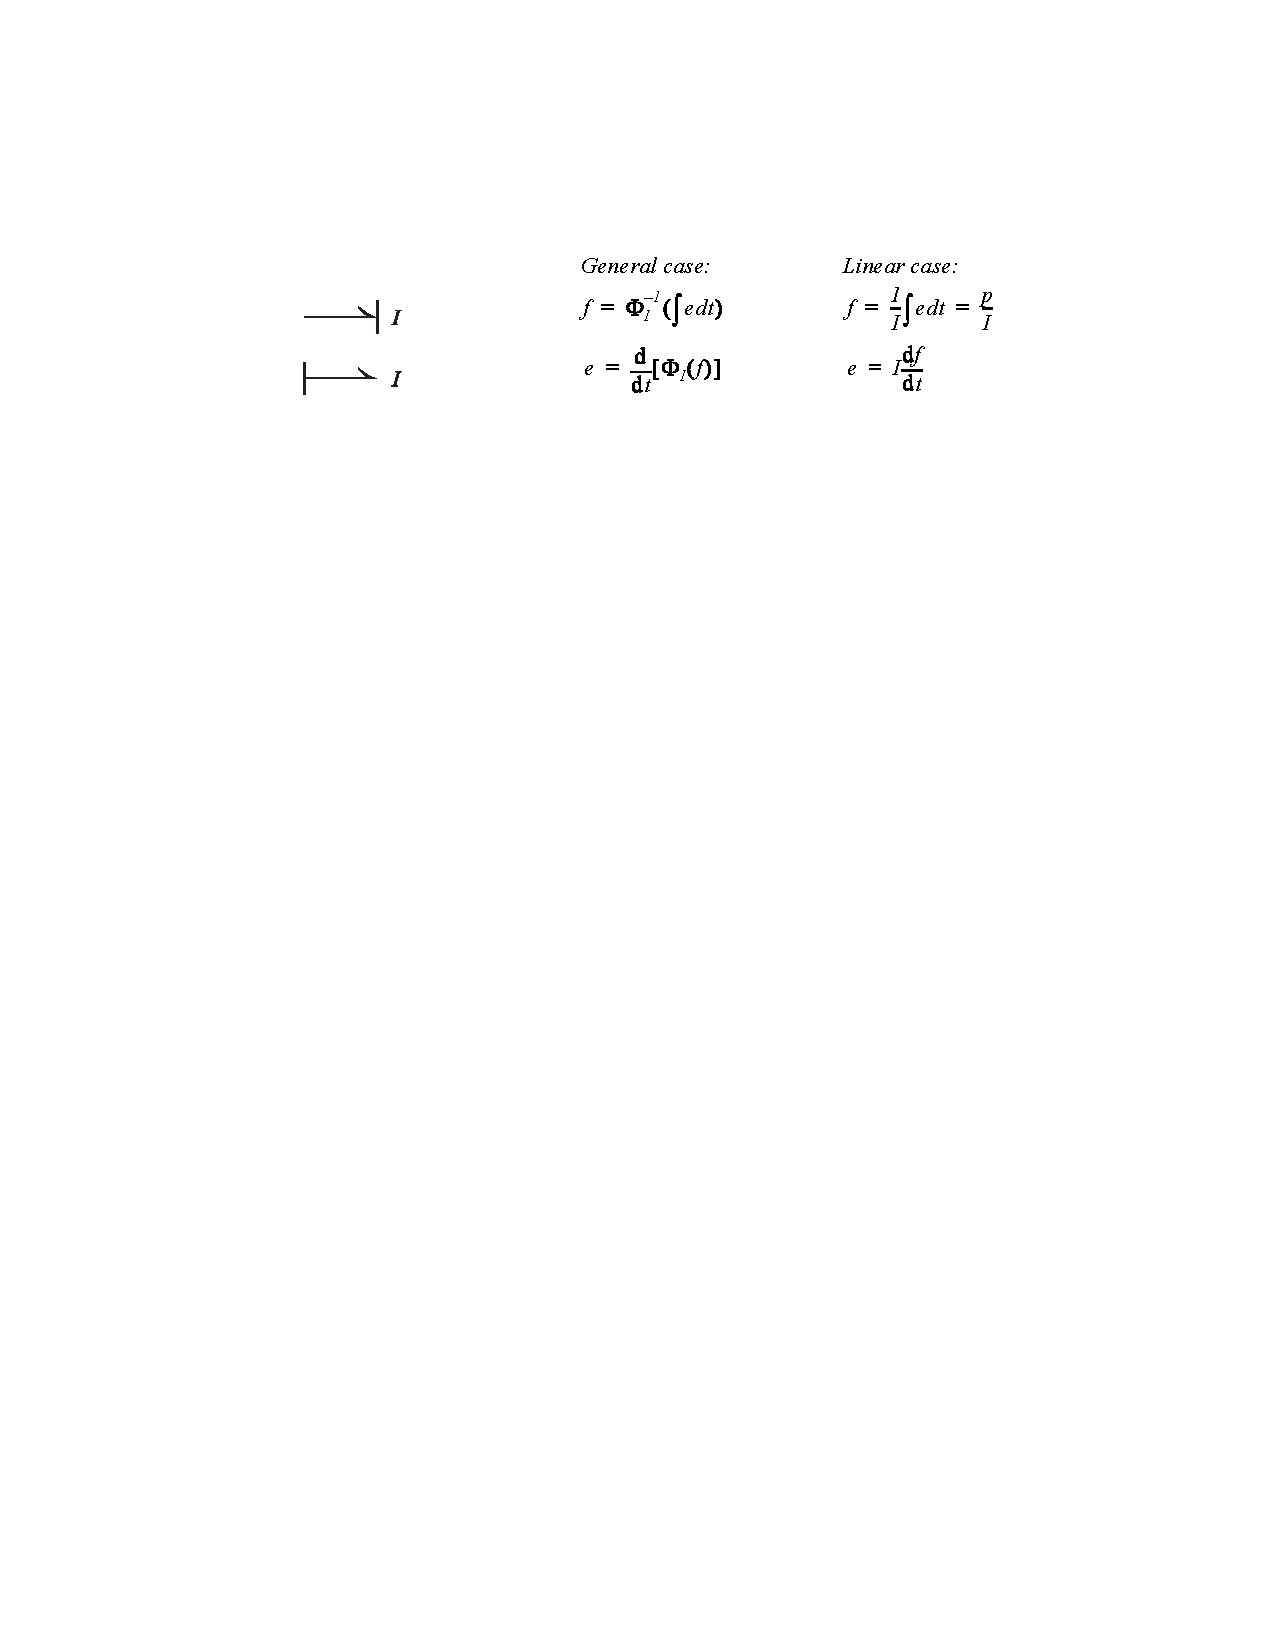
\includegraphics[width=.9\linewidth]{figures/fig46.pdf}
        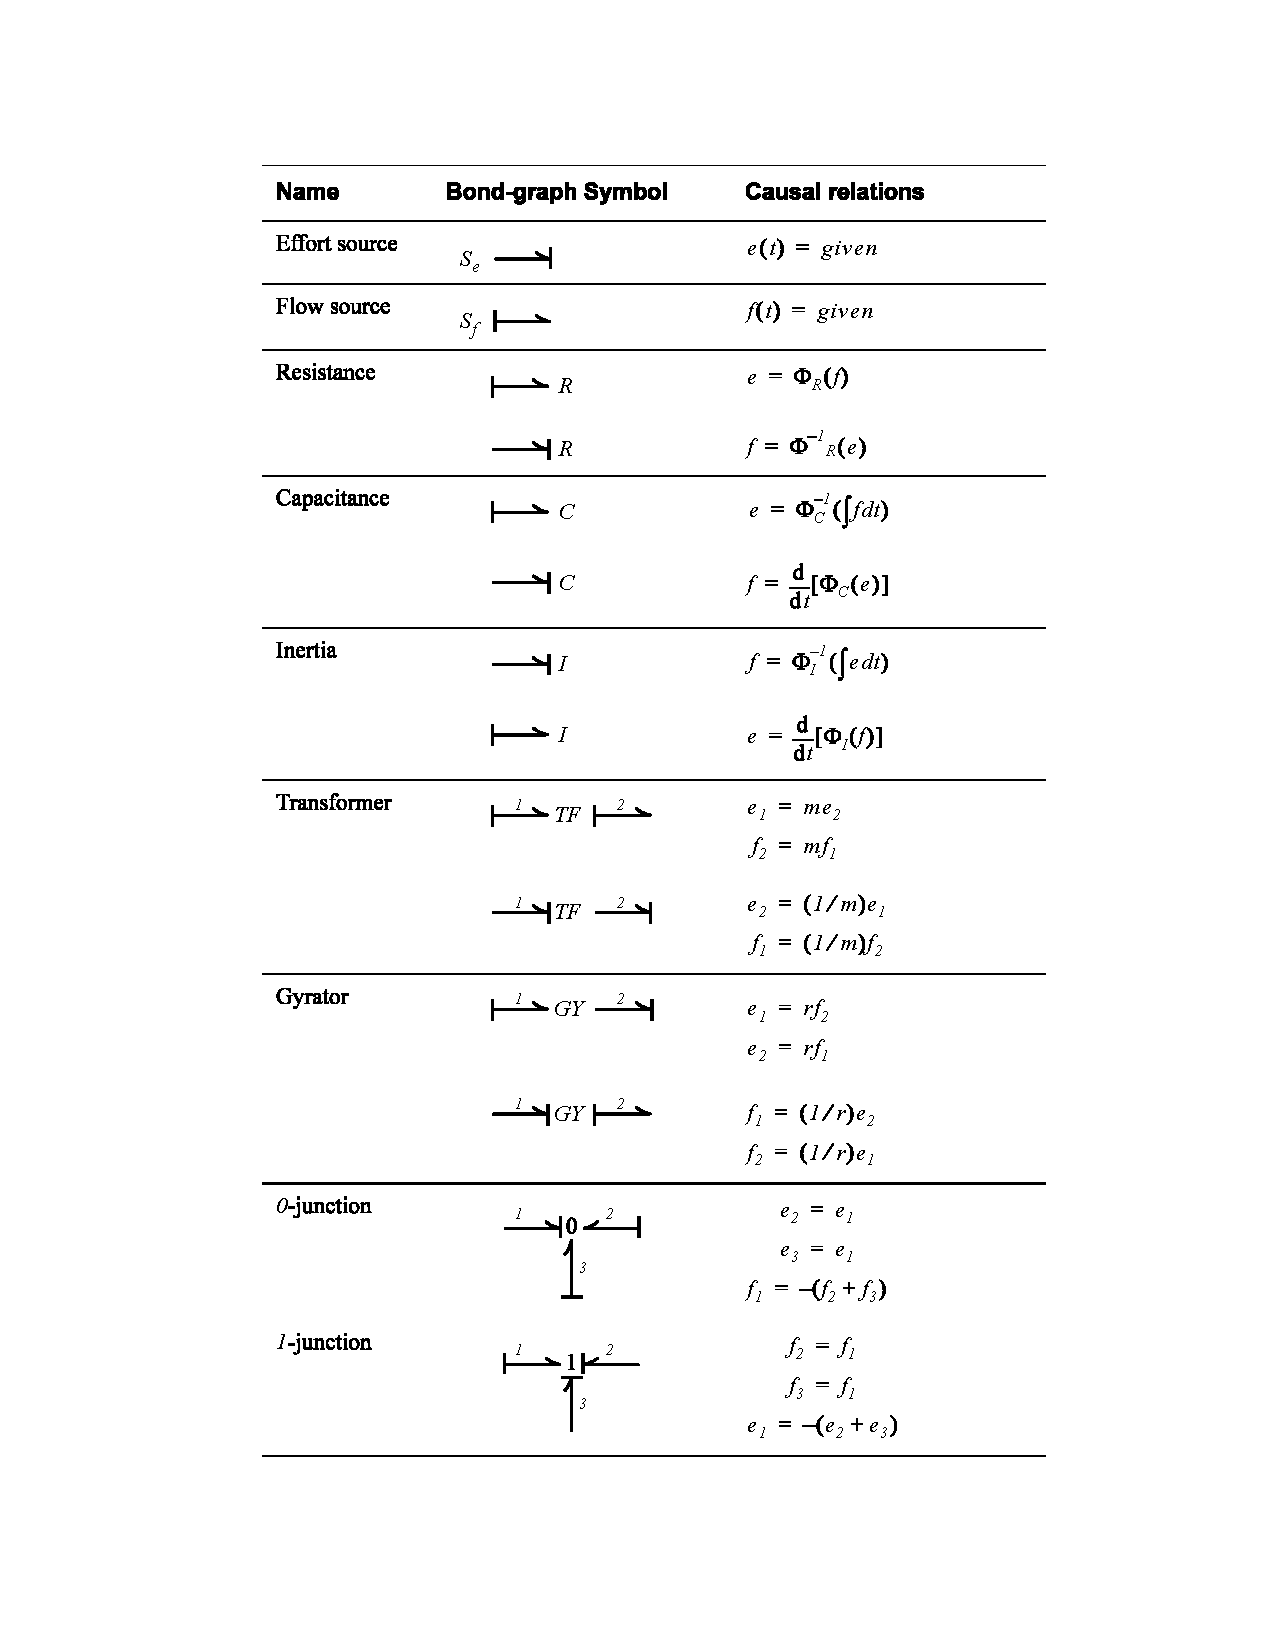
\includegraphics[width=.9\linewidth]{figures/Tabell_CausalRelations.pdf}
        \label{fig:bond_graph3}
        \fbox{\parbox{\linewidth}{
            \textbf{Generally:}\newline
            $p(t) = \int_{0}^{t} e(t)\,dt + p(0) \Rightarrow \dot{p} = e$\newline
            $q(t) = \int_{0}^{t} f(t)\,dt + q(0)  \Rightarrow \dot{q} = f$\newline
            $P(t) = e(t)f(t), \quad E(t) = \int_{0}^{t} P(t) \,dt = \int_{0}^{t} e(t)f(t) \,dt$
        }}
    \end{minipage}
\end{figure}
\textbf{Finding state-space model: }\newline
For all $I$ and $C$ elements with integral causality, set your states $\mathbf{x} = [p_i, p_j, q_k, q_l]$, where $i,j,k,l$ are the indices of the elements with integral causality. $I$ and $C$ elements with derivative causality are not part of your states!!
\newpage
\subsection{Drawing a bond graph}
\textbf{From the book: }
\begin{enumerate}
    \item Since the velocity is the same at any connection point between elements, then establish a 1-junction for each distinct velocity.
    \item Add existent inertia and capacitance elements to their respective 1-junctions.
    \item Add resistance elements to their respective 0- and 1-junctions.
    \item Add transformation and gyrator elements between junctions.
    \item For each 1-port element establish the relative velocity over the element by bonding a 0-junction between appropriate 1-junctions. Adjoin the pertinent 1-port element to the 0-junction.
    \item Remove all 1-junctions with zero velocity and all the bonds connected to these 1-junctions.
    \item Assign power directions on all bonds.
    \item Simplify the bond graph by replacing 2-port 0- and 1-junctions with through power directions by single bonds.
    \item Add causality to the elements.
\end{enumerate}
\textbf{Based on the school of life: }
Start by finding the velocities in your system. This means translational and rotational velocities. (This is of course talking about mechanical systems. If you find your self having to model a system that is electrical, it will be pretty simple to use the table on the previous page. If you find your self having to model a hydraulic system on the other hand, themn you are pretty fucked. Let's hope you don't)
The easiest way to do this, is finding an expression for the position, then differentiating with respect to time. You will then hopefully be able to find a relation between rotation and translation, and maybe even relation between rotation and rotation or translation and translation. Remember to assign inertia elements to most velocities. If your velocity is translational, it will most likely be $I : m$